\documentclass[aspectratio=169]{beamer}
 % For widescreen (16:9)
%\documentclass[aspectratio=43]{beamer}  % For standard (4:3)

\usetheme{Madrid}
\usecolortheme{default}

\title{A study on age, gender, and race classification from facial images using deep convolutional neural networks (CNNs) with transfer learning}

\date

% Define the contents
\newcommand{\contents}{
    \footnotesize
        Student ID: 22031359 \newline
        Module: Data Science Project \newline
        Supervisor: Dr. Darshan Kakkad
}

\author{Dileepa Joseph Jayamanne}

\date % (optional)

\definecolor{uoftblue}{RGB}{6,41,88}
\setbeamercolor{titlelike}{bg=uoftblue}
\setbeamerfont{title}{series=\bfseries}

% Put other packages here:
\usepackage{geometry}
\usepackage{tabularx}
\usepackage{array}
\usepackage{multirow}
\usepackage{colortbl}
\usepackage{xcolor}
\usepackage{graphicx}
\usepackage{tcolorbox} % For colored boxes

\usepackage{overpic}
\usepackage{lipsum} 
%\usepackage{caption}
%\usepackage{adjustbox}

\usepackage{hyperref}
\usepackage{ulem}
% \hypersetup{
%       colorlinks=true,
%       linkcolor=blue,
%       filecolor=blue,
%       urlcolor=blue,
%       citecolor=blue
% }

\begin{document}

%-------- Slide 1 - Title page ---------------------
\frame{\titlepage 
\vspace{-1.75cm} % Adjust the vertical space here
\contents

%\vfill % Pushes the URLs to the bottom
%    \footnotesize
%    \textbf{GitHub URL:} 
%    \textcolor{blue}{\href{https://github.com/7PAM2015-0509-2023-Team4/Kaggle-Challenge}{https://github.com/7PAM2015-0509-2023-Team4/Kaggle-Challenge}} \\
%    \textbf{Colab URL:} \textcolor{blue}{\href{https://colab.research.google.com/drive/1n0WzVOPsseVm8f8Qpydyvd-iCqEw0vDN?usp=sharing}{https://colab.research.google.com/drive/1n0WzVOPsseVm8f8Qpydyvd-iCqEw0vDN?usp=sharing}}
    
}

% ------- Slide 2: Table of Contents -----------------
\begin{frame}
\frametitle{Table of Contents}
\tableofcontents
\end{frame}

\section{Introduction}
% ------- Slide 3: ----------------------------
\begin{frame}
\frametitle{Introduction: Task and Application}
   \begin{alertblock}{Task}
     To extract demographic information from facial images.
    \end{alertblock}
    \vfill
    \begin{exampleblock}{Applications}
    \begin{itemize}
        \item Businesses can promote advertising for an identified target group of potential customers online.
        \item Law and enforcement can track down a suspect quickly given the surveillance footage of people and some prior demographic information.
    \end{itemize}
    \end{exampleblock}
\end{frame}

\section{Research Question and Objectives}
% ------- Slide 4: ----------------------------
\begin{frame}
\frametitle{Research Question and Objectives}
\textbf {Research Question:}
\begin{itemize}
    \item How accurately can deep CNNs with transfer learning classify age, gender and race from facial images?
\end{itemize}
\vfill 
\textbf {Research Objectives:}
\begin{itemize}
    \item To classify facial images into age groups, gender, and race using deep CNNs with transfer learning.
    \item To investigate if gender could be used as a prior in age classification for improved performance.
\end{itemize}
\end{frame}


\section{Overview of the Dataset}
% ------- Slide 5: ----------------------------
\begin{frame}
\frametitle{Overview of the Dataset}
\begin{table}[h]
\centering
\begin{tabular}{|l|l|}
\hline
\textbf{Field}     & \textbf{Description} \\ \hline
Dataset            & UTKFace               \\ \hline
Authors            & Zhifei Zhang, Yan Song, and Hairong Qi \\ \hline
Location           & University of Tennessee Knoxville \\ \hline
Data               & 20k images of faces in jpg format (1.3 GB) \\ \hline
Labels             & Age, gender, and ethnicity \\ \hline
Image Details      & Size varies with different poses and illumination \\ \hline
\end{tabular}
\caption{Details of the UTKFace Dataset}
\end{table}
\end{frame}

\section{Exploratory Data Analysis of UTKFace}
% ------- Slide 6: ----------------------------
\begin{frame}
\frametitle{Age group distribution in UTKFace}
\begin{figure}
    \centering
    \includegraphics[scale=0.50]{fig1_age_distribution.png}
    \caption{Age group distributions}
    \label{fig1}
\end{figure}
\end{frame}

% ------- Slide 7: ----------------------------
\begin{frame}
\frametitle{Donut chart for gender and race}
\begin{figure}
    \centering
    \includegraphics[width=60mm,scale=0.60]{fig2_donut.png}
    \caption{Gender and race percentages}
    \label{fig2}
\end{figure}
\end{frame}

% ------- Slide 8: ----------------------------
\begin{frame}
\frametitle{Race distributions in UTKFace}
\begin{figure}
    \centering
    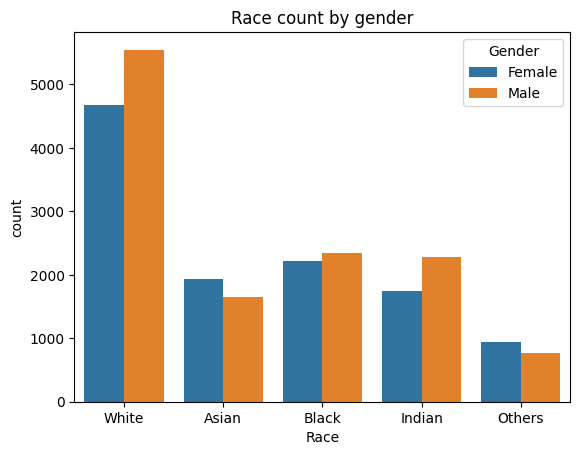
\includegraphics[scale=0.50]{fig3_race_count.png}
    \caption{Race count by gender}
    \label{fig3}
\end{figure}
\end{frame}

\section{Methodology}
% ------- Slide 9: ----------------------------
\begin{frame}
\frametitle{Methodology}
\begin{exampleblock}{}
  \begin{itemize}
  \setlength\itemsep{1em} 
    \item Detect and extract faces from the original dataset using Viola \& Jones technique (2001) or RetinaFace (Deng et al., 2020) - A deep learning approach.
    \item Use at least 3 base models - VGG16 (Simonyan and Zisserman, 2015), Resnet50 (He et al., 2016), and EfficientNet (Tan and Le, 2020) trained on ImageNet.
    \item Attach a classifier head to the base network and retrain the classifier head and some of the latter layers in the base network on the face data to build classifiers.
  \end{itemize}
\end{exampleblock}
\end{frame}

% ------- Slide 10: ----------------------------
\begin{frame}
\frametitle{VGG-model used in an experiment on gender classification}
\begin{figure}
    \centering
    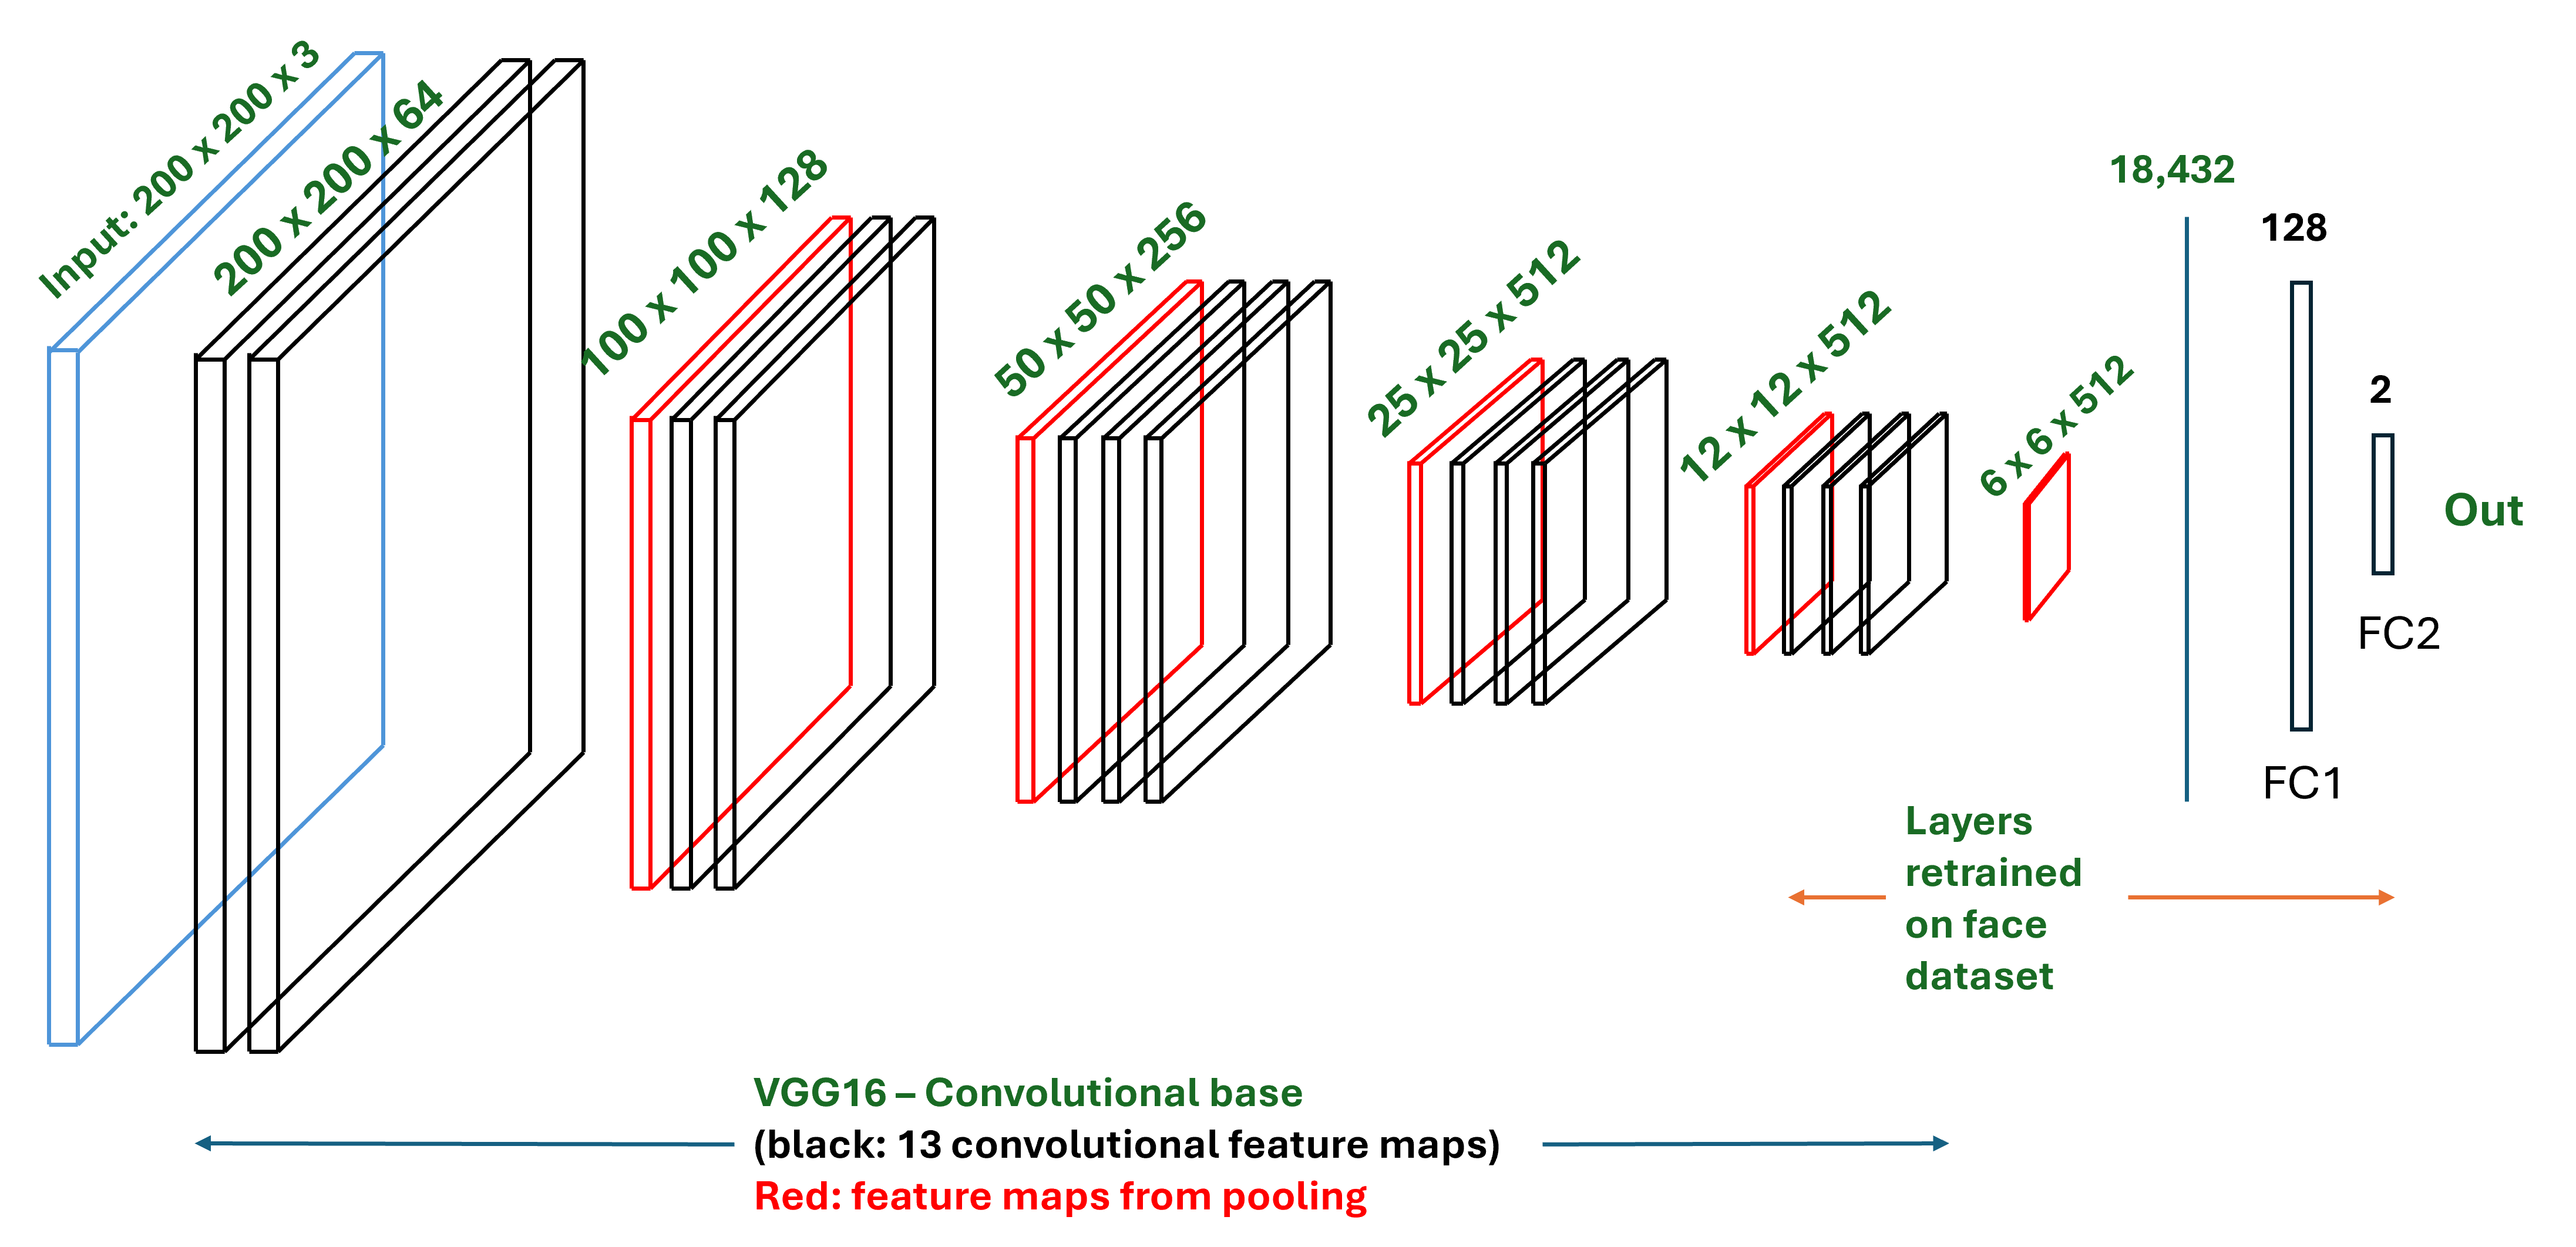
\includegraphics[scale=0.40]{fig4_VGGmodel.png}
    %\caption{VGG model used}
    \label{fig4}
\end{figure}
The above figure is author-generated.
\end{frame}

% ------- Slide 11: ----------------------------
\begin{frame}
\frametitle{Training and Validation Results on Gender Classification}
\begin{figure}
    \centering
    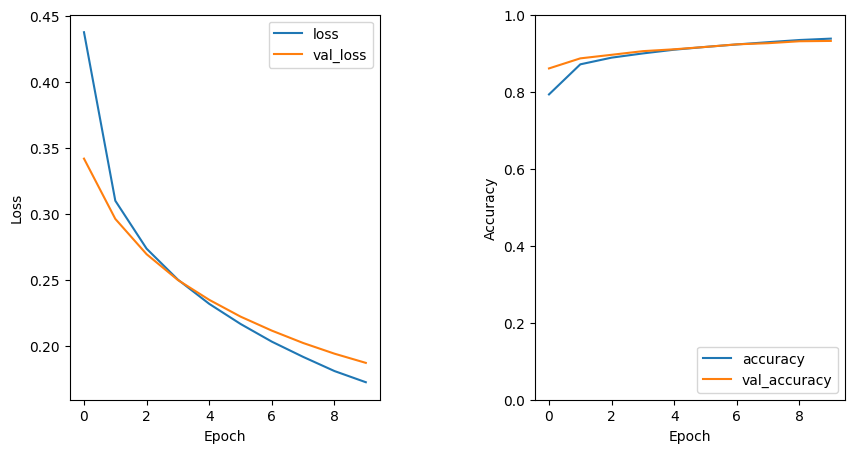
\includegraphics[scale=0.50]{fig5_learning_curve.png}
    \caption{Left: Training and validation losses. Right: Training and validation accuracies. Following observations were made in the 10th epoch: training loss= 0.1718, validation loss= 0.1871, training accuracy= 0.9374, validation accuracy= 0.9319 }
    \label{fig6}
\end{figure}
\end{frame}

\section{Ethical Requirement and Document Storage}
% ------- Slide 12: ----------------------------
\begin{frame}
\frametitle{Ethical Requirement and Document Storage}
\begin{exampleblock}{Ethical Considerations}
\begin{itemize}
    \item According to the author’s website, the UTKFace dataset can be used for non-commercial research work.
    \item No face is annotated with actual names.
    \item No exact age of a person will be estimated.
\end{itemize}
\end{exampleblock}
\vfill
\begin{block}{Document Storage}
\begin{itemize}
    \item The Colab files and data will be stored in GitHub, Google Drive, and University One Drive. 
    \item The files will be backed up weekly. 
\end{itemize}
\end{block}

\end{frame}

\section{Project Timeline}
% ------- Slide 13: ----------------------------
\begin{frame}
\frametitle{Project Timeline}
\begin{figure}
    \centering
    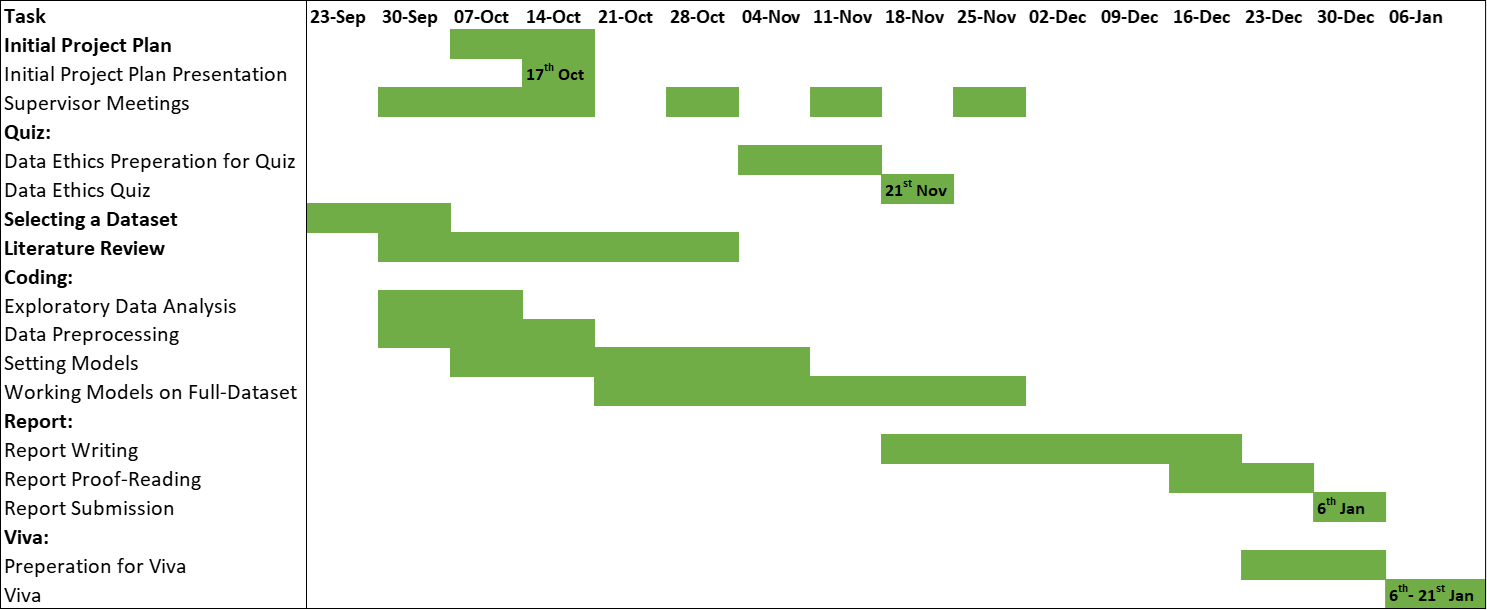
\includegraphics[scale=0.58]{fig6_timeline.png}
    %\caption{}
    \label{fig4}
\end{figure}
\end{frame}

% ------- Slide 14: ----------------------------
\begin{frame}
\frametitle{References}
\footnotesize
Deng, J., Guo, J., Ververas, E., Kotsia, I. and Zafeiriou, S. (2020). RetinaFace: Single-Shot Multi-Level Face Localisation in the Wild. \textit{2020 IEEE/CVF Conference on Computer Vision and Pattern Recognition (CVPR)}. Available at: \color{blue}
\url{https://doi.org/10.1109/cvpr42600.2020.00525}
\newline \newline
\color{black}
He, K., Zhang, X., Ren, S. and Sun, J. (2016). Deep Residual Learning for Image Recognition. In: \textit{Proceedings of the IEEE Conference on Computer Vision and Pattern Recognition (CVPR)}. IEEE, pp.770–778. Available at: 
\color{blue}
\url{https://doi.org/10.1109/cvpr.2016.90}
\newline \newline
\color{black}
Simonyan, K. and Zisserman, A. (2015). Very Deep Convolutional Networks for Large-Scale Image Recognition. \textit{Proceedings of the International Conference on Learning Representations (ICLR)}. ICLR. Available at: 
\color{blue}
\url{https://arxiv.org/abs/1409.1556}
\newline \newline
\color{black}
Tan, M. and Le, Q. (2020). \textit{EfficientNet: Rethinking Model Scaling for Convolutional Neural Networks}. [online] Available at: 
\color{blue}
\url{https://arxiv.org/pdf/1905.11946}
\newline \newline
\color{black}
Viola, P. and Jones, M. (2001). Rapid object detection using a boosted cascade of simple features. \textit{Proceedings of the IEEE Computer Society Conference on Computer Vision and Pattern Recognition (CVPR)}. Conference at Kauai, HI (USA), 8-14 December. IEEE Computer Society. Available at: 
\color{blue}
\url{https://doi.org/10.1109/cvpr.2001.990517}
\newline \newline
\color{black}
\end{frame}


% ------- Q & A ----------------------------
\begin{frame}
\frametitle{Questions and Answers}
  \begin{center}
    \begin{tcolorbox}[colback=blue!10!white, colframe=blue!75!black, width=\textwidth, sharp corners=south]
      \centering
      \Huge
      \textbf{Q \& A}
    \end{tcolorbox}
  \end{center}
\end{frame}

\end{document}







\section{Second section}
\begin{frame}
\frametitle{Highlighting text}

In this slide, some important text will be
\alert{highlighted} because it's important.
Please, don't abuse it.

\begin{block}{Remark}
Sample text
\end{block}

\begin{alertblock}{Important theorem}
Sample text in red box
\end{alertblock}

\begin{examples}
Sample text in green box. The title of the block is ``Examples".
\end{examples}
\end{frame}

\end{document}
